%%% Design basiert auf:
%% LaTeX-Beamer template for KIT design
%% by Erik Burger, Christian Hammer
%% title picture by Klaus Krogmann
%% version 2.1
\documentclass[18pt]{beamer}

\usepackage{templates/beamerthemekit}
\usepackage{graphicx} %because it will be included below
\usepackage{listings}
%\usepackage{wasysym}
\usepackage{color}
\usepackage[T1]{fontenc}
%\usepackage{cmap}
\usepackage{textcomp}
\usepackage[utf8]{inputenc}
%\usepackage{pdfpages}
\definecolor{listinggray}{gray}{0.9}
\definecolor{lbcolor}{rgb}{0.9,0.9,0.9}
\lstset{
        language=Java,
        backgroundcolor=\color{lbcolor},
        tabsize=4,
		keepspaces,
		extendedchars=true,
        rulecolor=\color{black},
        basicstyle=\footnotesize,
        aboveskip=0pt,
        upquote=true,
        columns=fixed,
        showstringspaces=false,
        extendedchars=true,
        breaklines=true,
        frame=single,
        showtabs=false,
        showspaces=false,
        showstringspaces=false,
        identifierstyle=\ttfamily,
        keywordstyle=\color[rgb]{0,0,1},
        commentstyle=\color[rgb]{0.133,0.545,0.133},
        stringstyle=\color[rgb]{0.627,0.126,0.941},
}


%% TITLE PICTURE
\titleimage{frontpic}


% For the title page
\title[Proggen WS11/12]{Programmieren WS 2011/2012}
\subtitle{Tutorium Nr. 1 / 11}
\author{Tobias Sturm} %, David Kulicke
\institute{Zertifizierbare Vertrauenswürdige Informatiksysteme}
\date[23.1.12] %TODO aktualisieren

% the presentation starts here
\begin{document}
\selectlanguage{ngerman}


%title page
\begin{frame}
	\titlepage
\end{frame}


%table of contents
\begin{frame}{Heute:}
%	\setcounter{tocdepth}{1}
	\tableofcontents
\end{frame}

\setbeamercovered{invisible}

%%%%%%%%%%%%%%%%%%%%%%%%%%%%%%%%%%%%%%%%%%%%%%%%%%%%%%%%%%%%%%%%%%%%%%%%%
%%%%%%%%%%%%%%%%%%%%%%%%%%%%%%%%%%%%%%%%%%%%%%%%%%%%%%%%%%%%%%%%%%%%%%%%%
%%%%%%%%%%%%%%%%%%%%%%%%%%%%%%%%%%%%%%%%%%%%%%%%%%%%%%%%%%%%%%%%%%%%%%%%%
\section*{Informationen}
\begin{frame}{Info}
	\begin{columns}[T]
		 \begin{column}{5cm}
			
\includegraphics[scale=1.5]{bilder/eulenfest.png}		 
		 \end{column}
 		 \begin{column}{5cm}
			\textbf{Eulenfest}
			\begin{itemize}
				\item organisiert von Ersties
				\item hier im Infobau
				\item Tanzmatten und Zuckerwatte
				\item Helfer gesucht (v.A. Auf-/Abbau)
			\end{itemize}
 		 \end{column}
	\end{columns}
\end{frame}

\begin{frame}{Infos}
	\textbf{Außerdem noch wichtig:}
	\begin{itemize}
		\item VL wird nicht mehr in HS -102 übertragen\pause
		\item Schreibt nicht ab (z.B. von Github)!\pause
		\item Heute in einem Jahr geht die Welt unter - genießt das letzte Jahr\pause
	\end{itemize}
\end{frame}

%%%%%%%%%%%%%%%%%%%%%%%%%%%%%%%%%%%%%%%%%%%%%%%%%%%%%%%%%%%%%%%%%%%%%%%%%
%%%%%%%%%%%%%%%%%%%%%%%%%%%%%%%%%%%%%%%%%%%%%%%%%%%%%%%%%%%%%%%%%%%%%%%%%
%%%%%%%%%%%%%%%%%%%%%%%%%%%%%%%%%%%%%%%%%%%%%%%%%%%%%%%%%%%%%%%%%%%%%%%%%
\section{Vererbung}
\subsection{Wozu?}
\begin{frame}{Vererbung - BirdSim}
	\begin{itemize}
		\item Simulator um Vögel zu simulieren: BirdSim
		\item Erstes Feature: Hintergrundgeräusche ausgeben. Alle bekannten Vögel sollen Geräusche machen.
		\item Dazu modellieren wir verschiedene Vögel in verschiedenen Klassen
	\end{itemize}

	\pause
	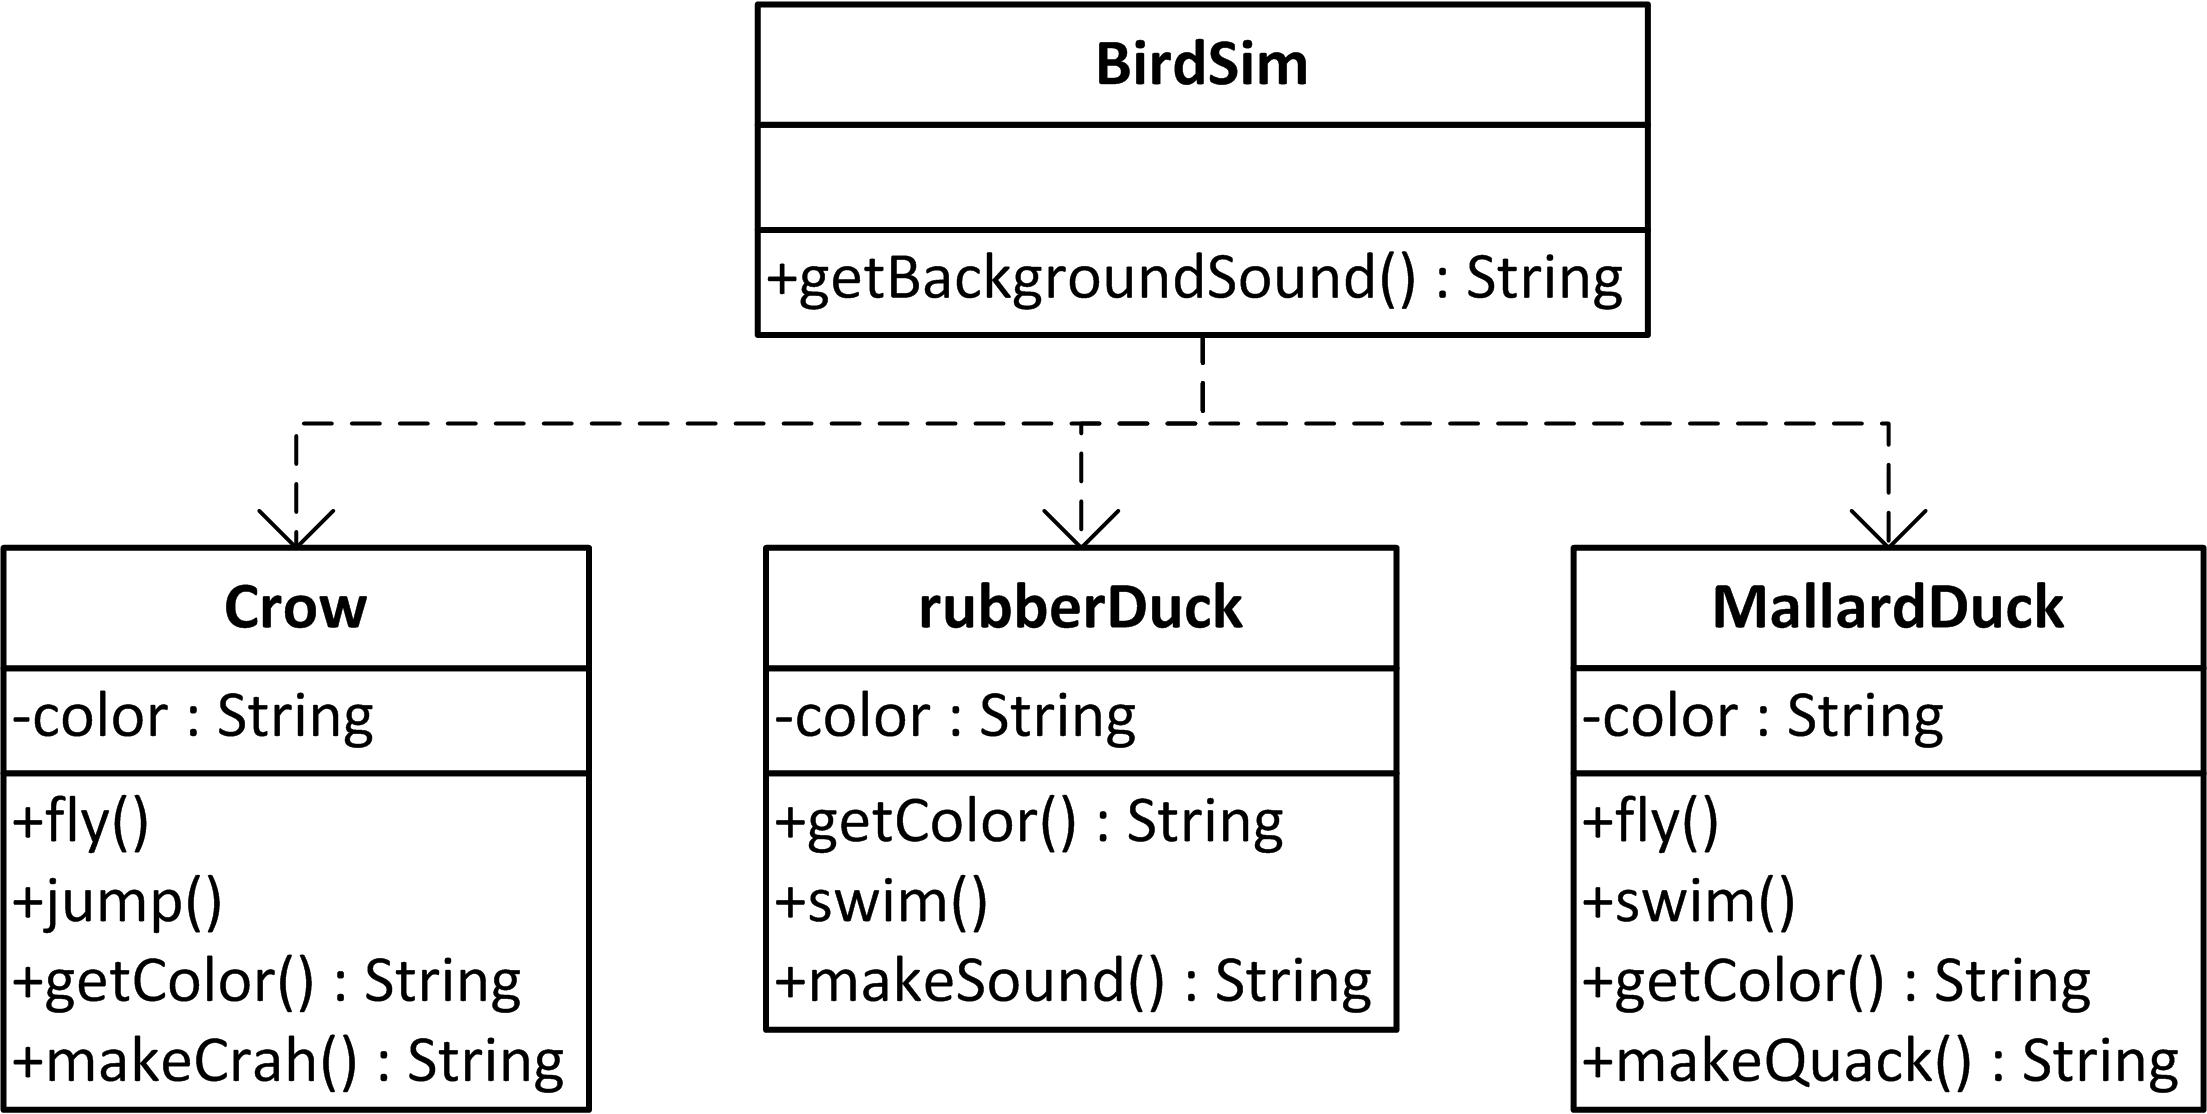
\includegraphics[scale=1]{bilder/uml/uml1.jpg}
\end{frame}

%%%%%%%%%%%%%%%%%%%%%%%%%%%%%%%%%%%%%%%%%%%%%%%%%%%%%%%%%%%%%%%%%%%%%%%%%

\begin{frame}{Vererbung - BirdSim}
	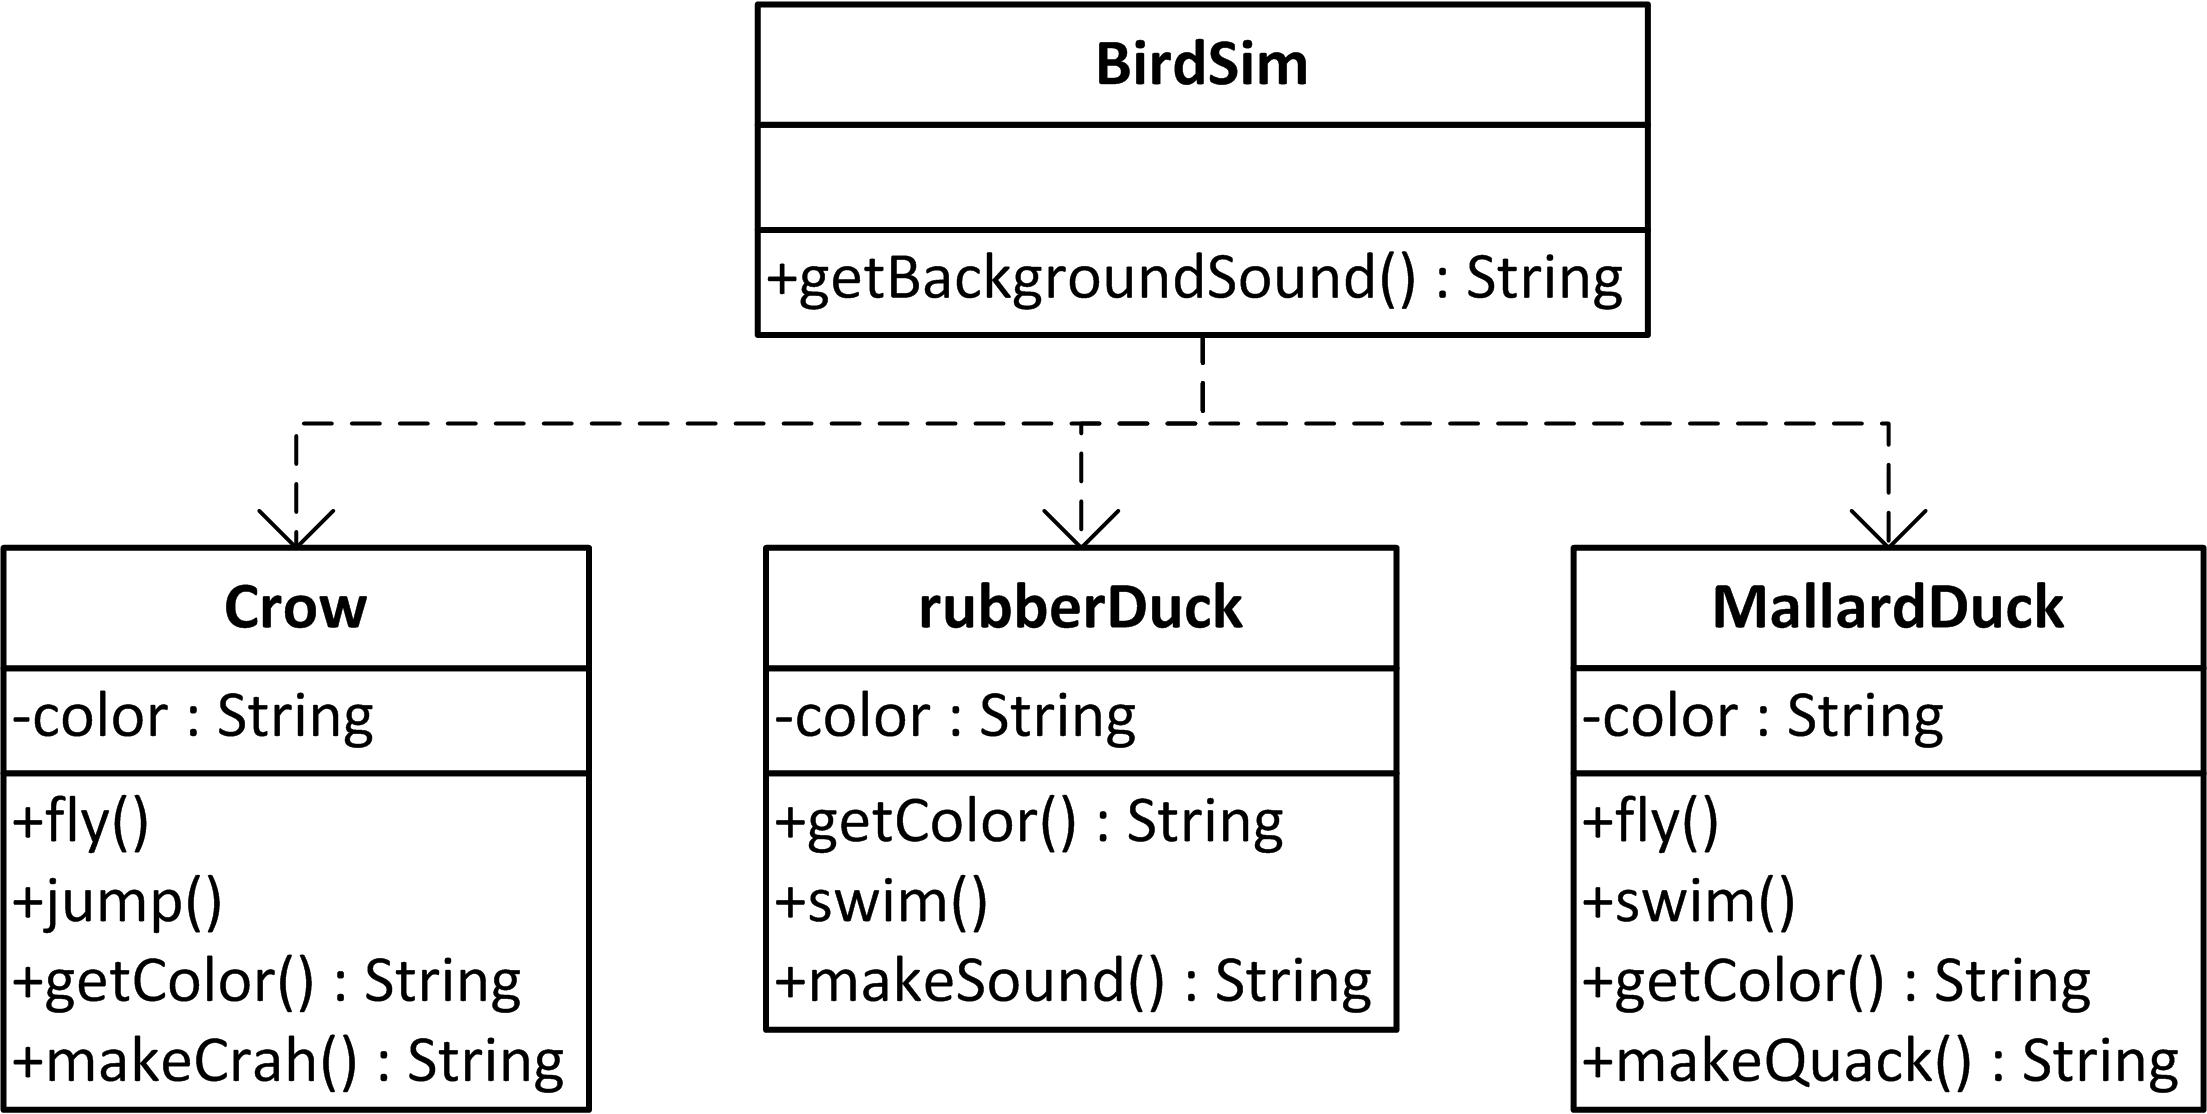
\includegraphics[scale=1]{bilder/uml/uml1.jpg}
	
	\textbf{Probleme:} 
	\begin{itemize}
		\item viele Abhängigkeiten
		\item \textit{getBackgroundSound} muss für jede neue Vogel-Klasse neu angepasst werden
		\item viele Dinge ähnlich
	\end{itemize}
	
	\emph{Hinweis: Diagramme werden nicht ganz korrekt sein}
\end{frame}

%%%%%%%%%%%%%%%%%%%%%%%%%%%%%%%%%%%%%%%%%%%%%%%%%%%%%%%%%%%%%%%%%%%%%%%%%

\begin{frame}{Vererbung - BirdSim}
	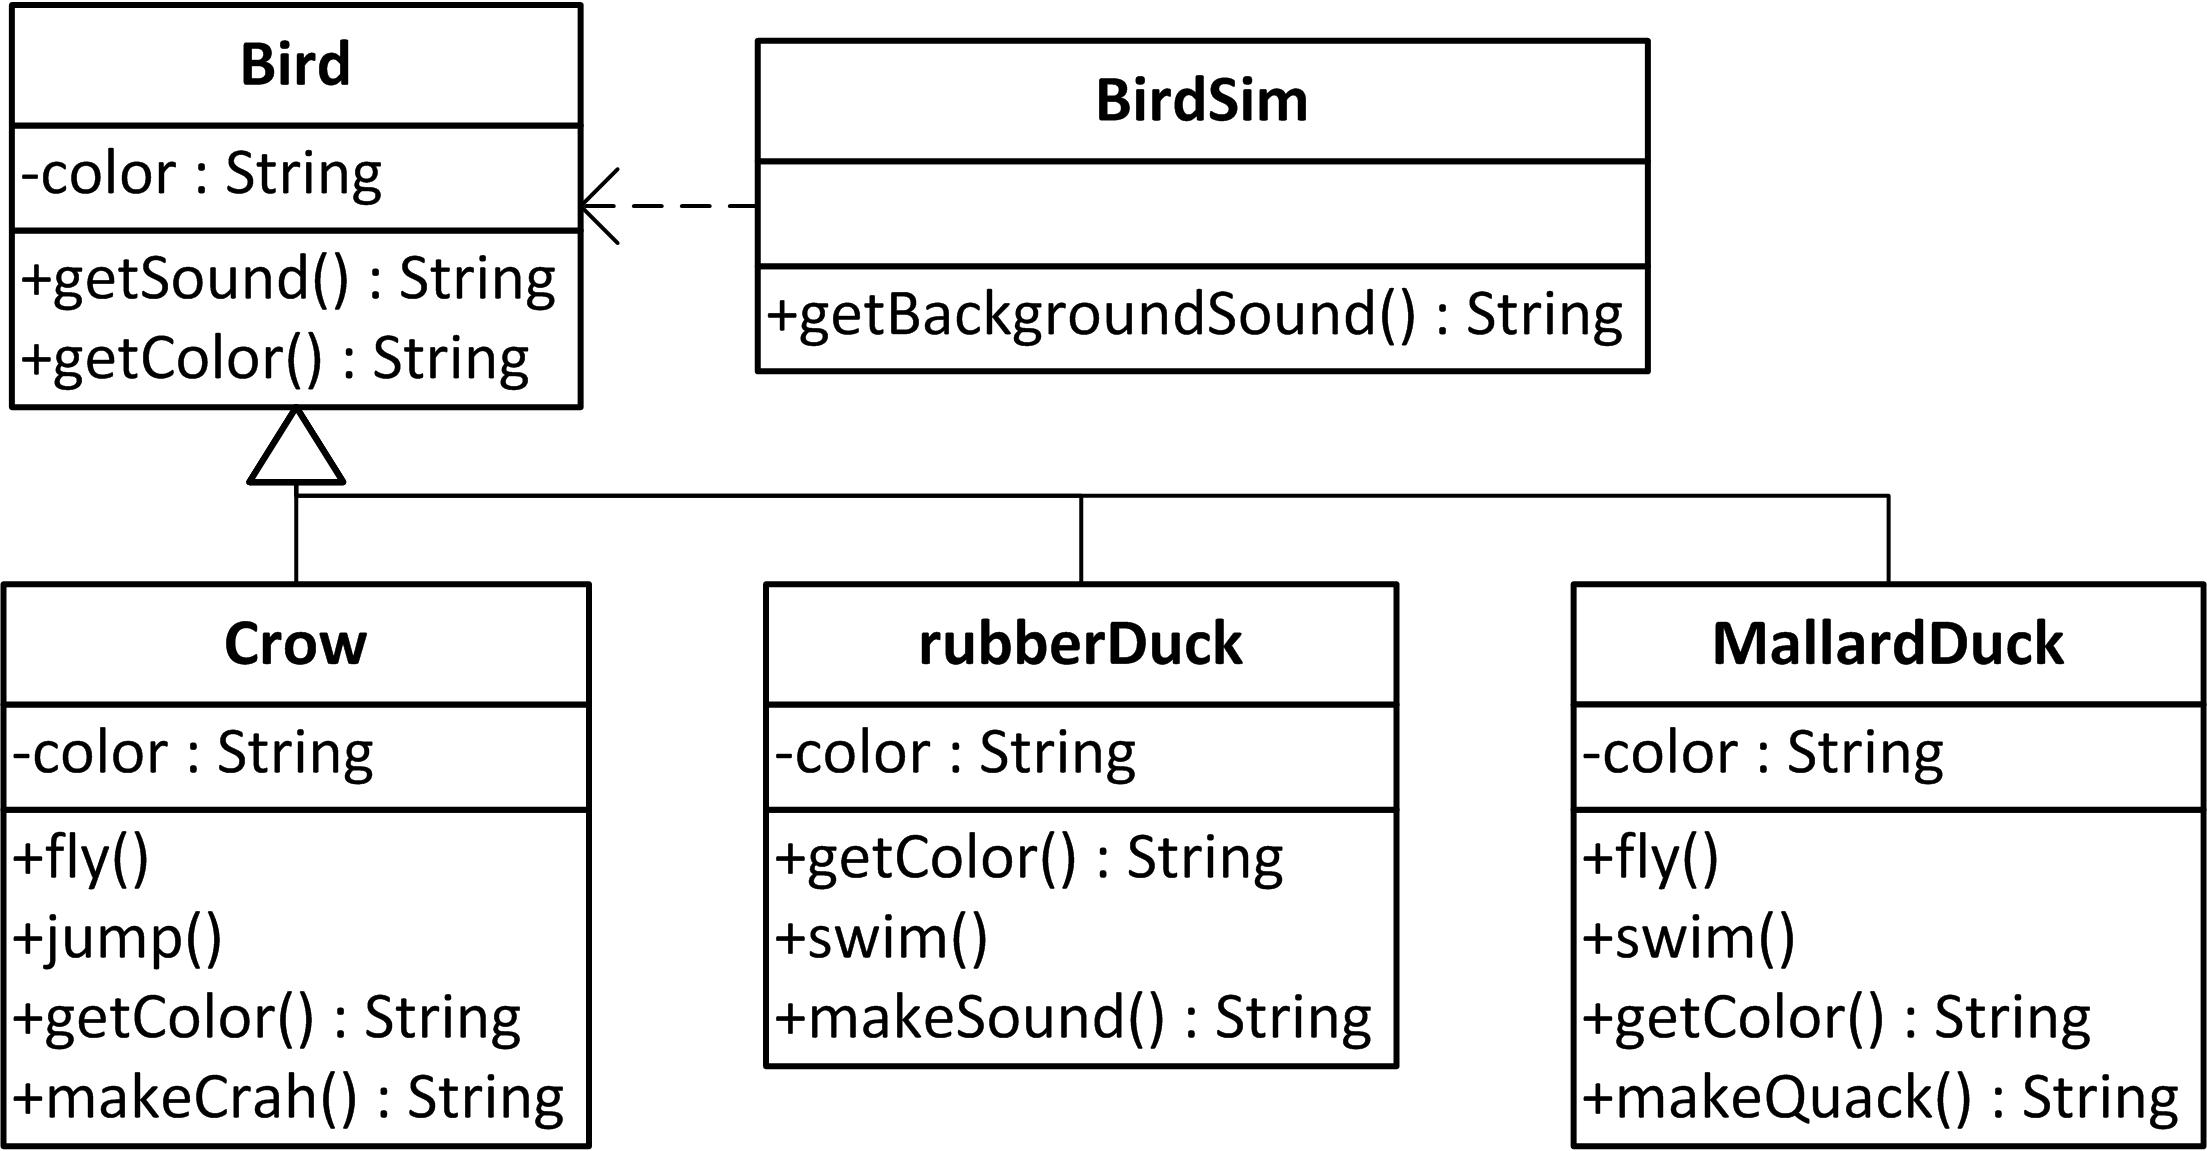
\includegraphics[scale=1]{bilder/uml/uml2.jpg}
	
	\textbf{Lösung:} Vererbung :)
	\begin{itemize}
		\item Jede Krähe ist ein Vogel
		\item Jede Stockente ist ein Vogel
		\item Jede Gummiente ist ein Vogel\pause
		\item Alle Vögel können Geräusche machen
	\end{itemize}
	
\end{frame}

%%%%%%%%%%%%%%%%%%%%%%%%%%%%%%%%%%%%%%%%%%%%%%%%%%%%%%%%%%%%%%%%%%%%%%%%%

\begin{frame}{Vererbung - BirdSim}
	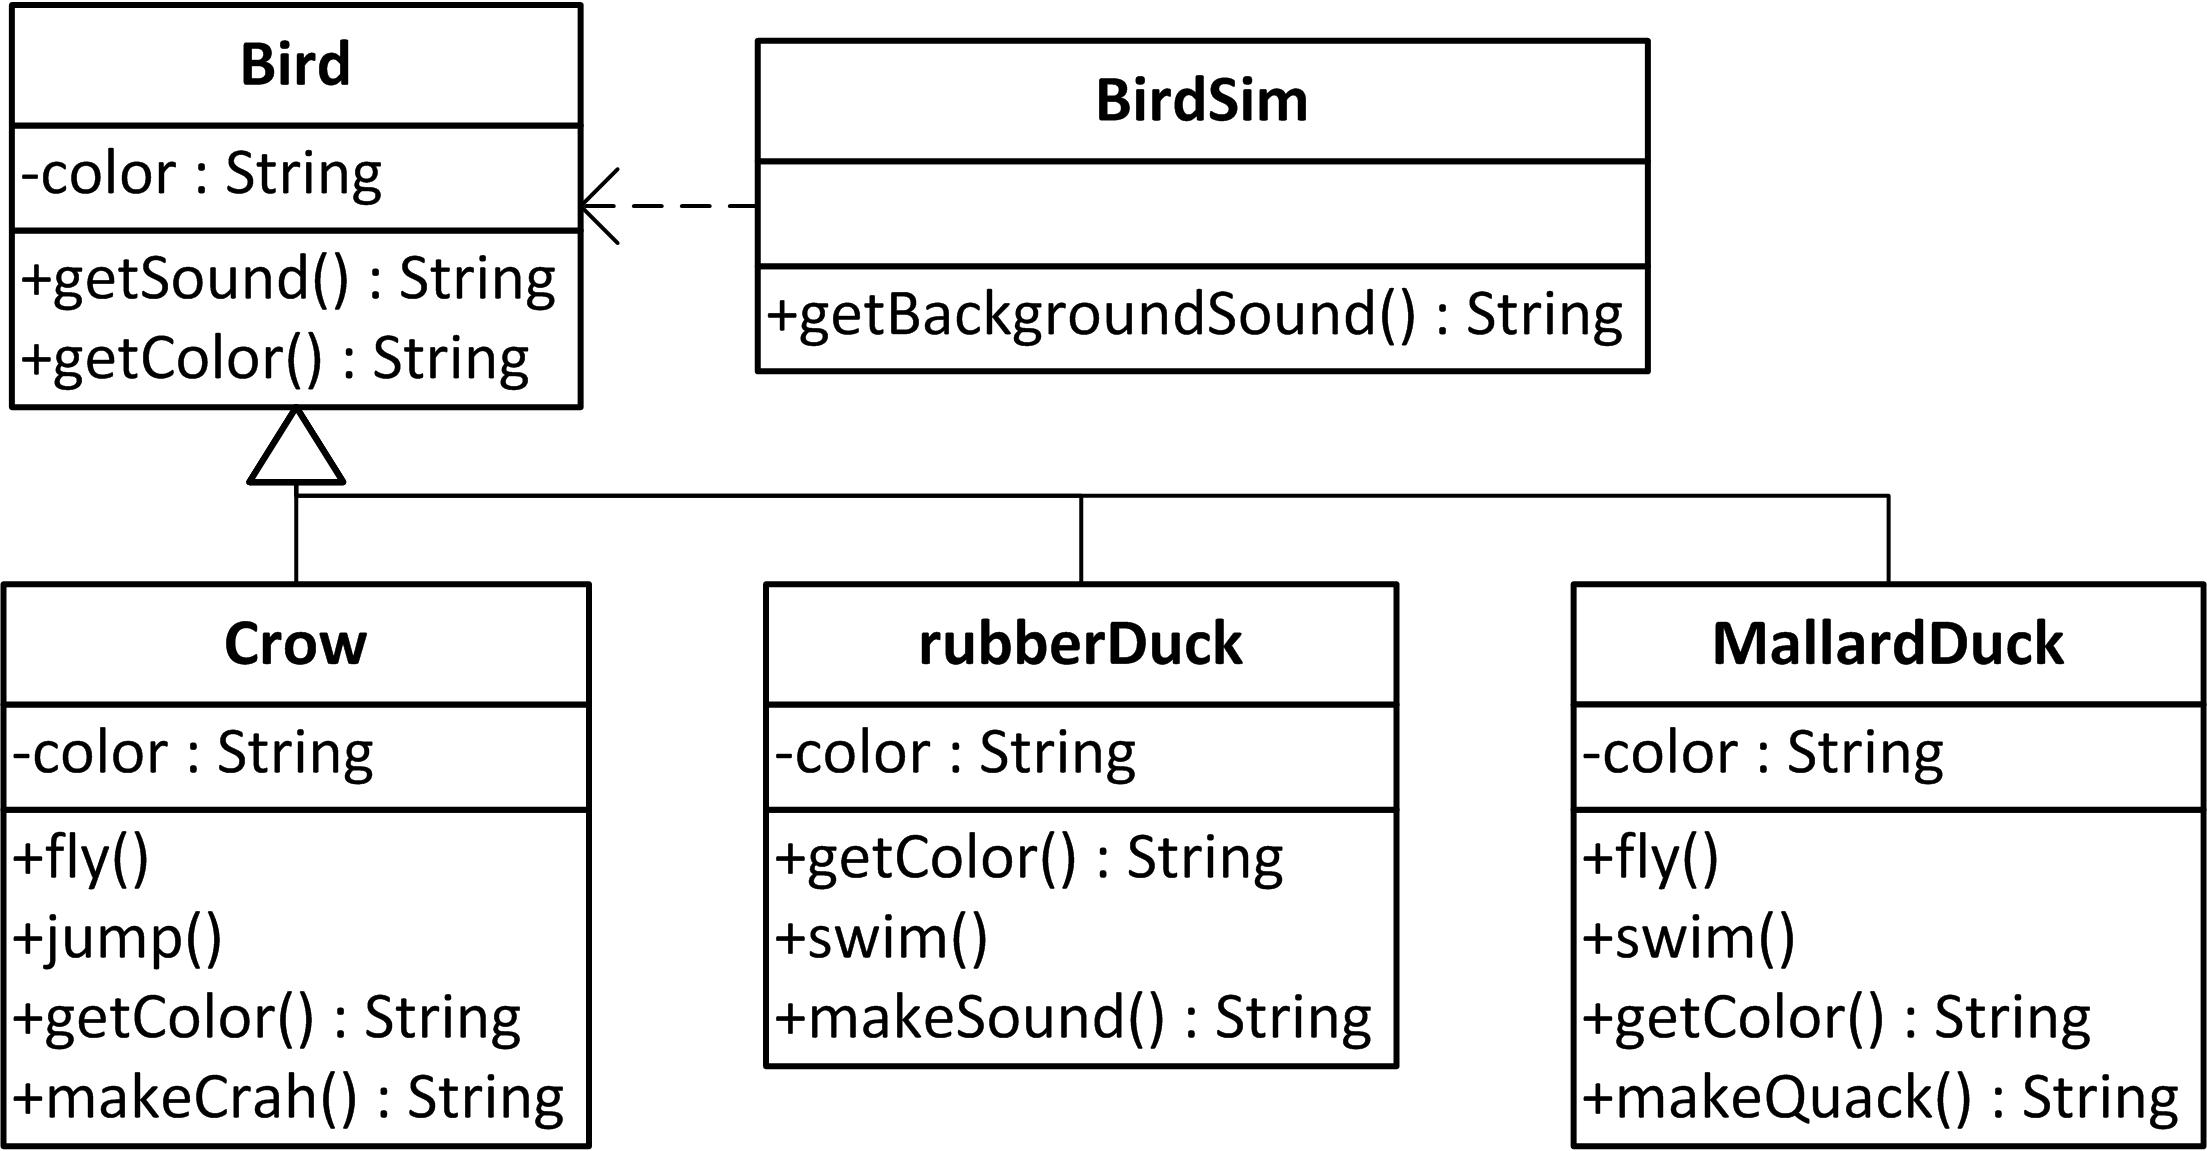
\includegraphics[scale=1]{bilder/uml/uml2.jpg}
	
	\textbf{Lösung:} Vererbung :)
	\begin{itemize}
		\item nicht alle Vögel können schwimmen
		\item nicht alle Vögel können fliegen
	\end{itemize}
\end{frame}

%%%%%%%%%%%%%%%%%%%%%%%%%%%%%%%%%%%%%%%%%%%%%%%%%%%%%%%%%%%%%%%%%%%%%%%%%

\begin{frame}{Vererbung - BirdSim}
	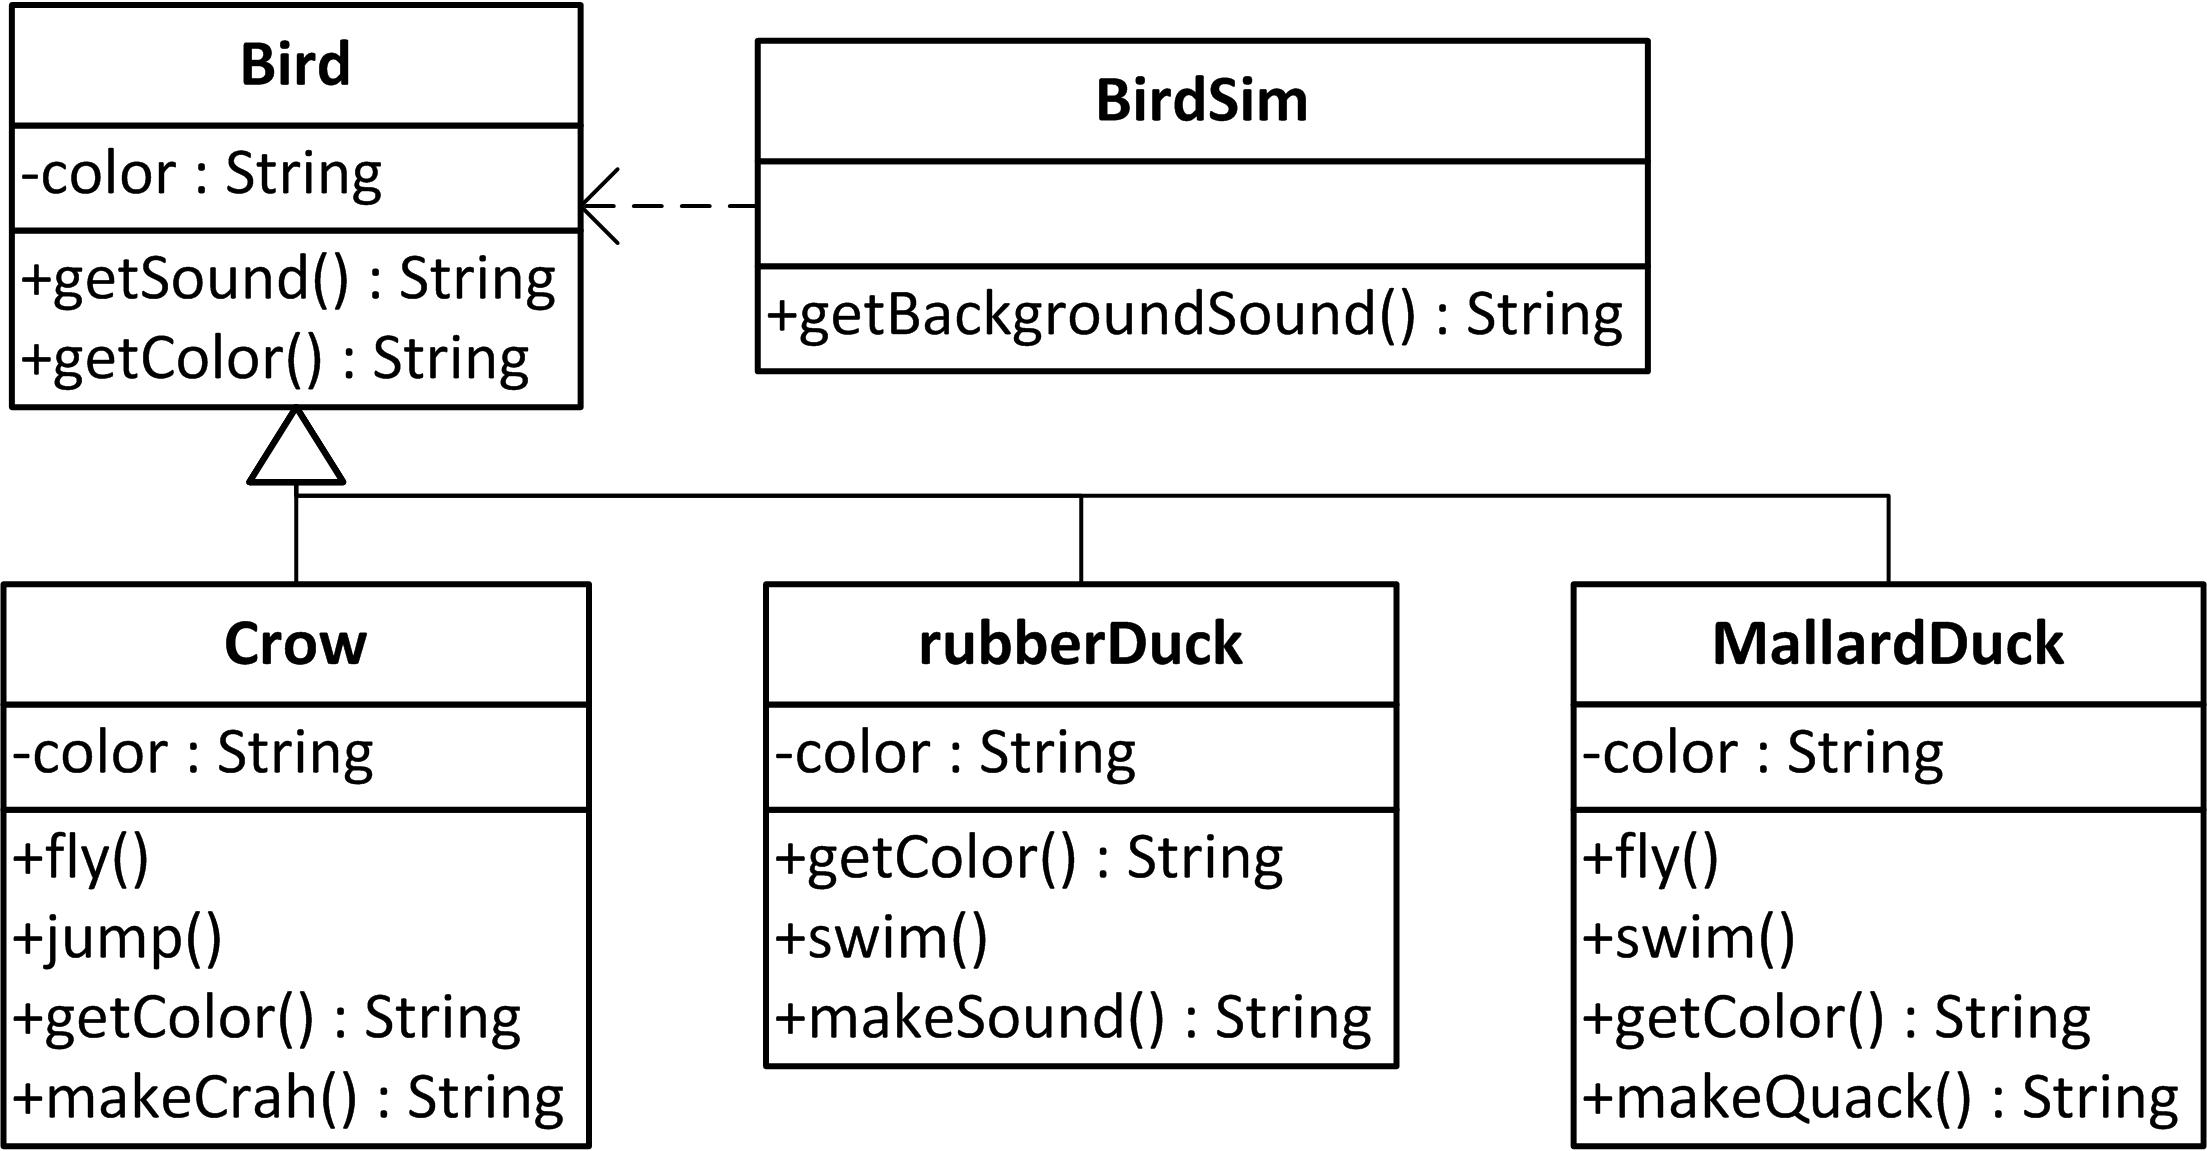
\includegraphics[scale=1]{bilder/uml/uml2.jpg}
	
	\textbf{Lösung:} Vererbung :)
	\begin{itemize}
		\item Attribute und Methoden werden übernommen
		\item Unterklassen können weitere Eigenschaften hinzufügen / verändern
	\end{itemize}\pause

	\textbf{Frage:} Kann man hier noch mehr vererben?
\end{frame}

%%%%%%%%%%%%%%%%%%%%%%%%%%%%%%%%%%%%%%%%%%%%%%%%%%%%%%%%%%%%%%%%%%%%%%%%%

\begin{frame}{Vererbung - BirdSim}
	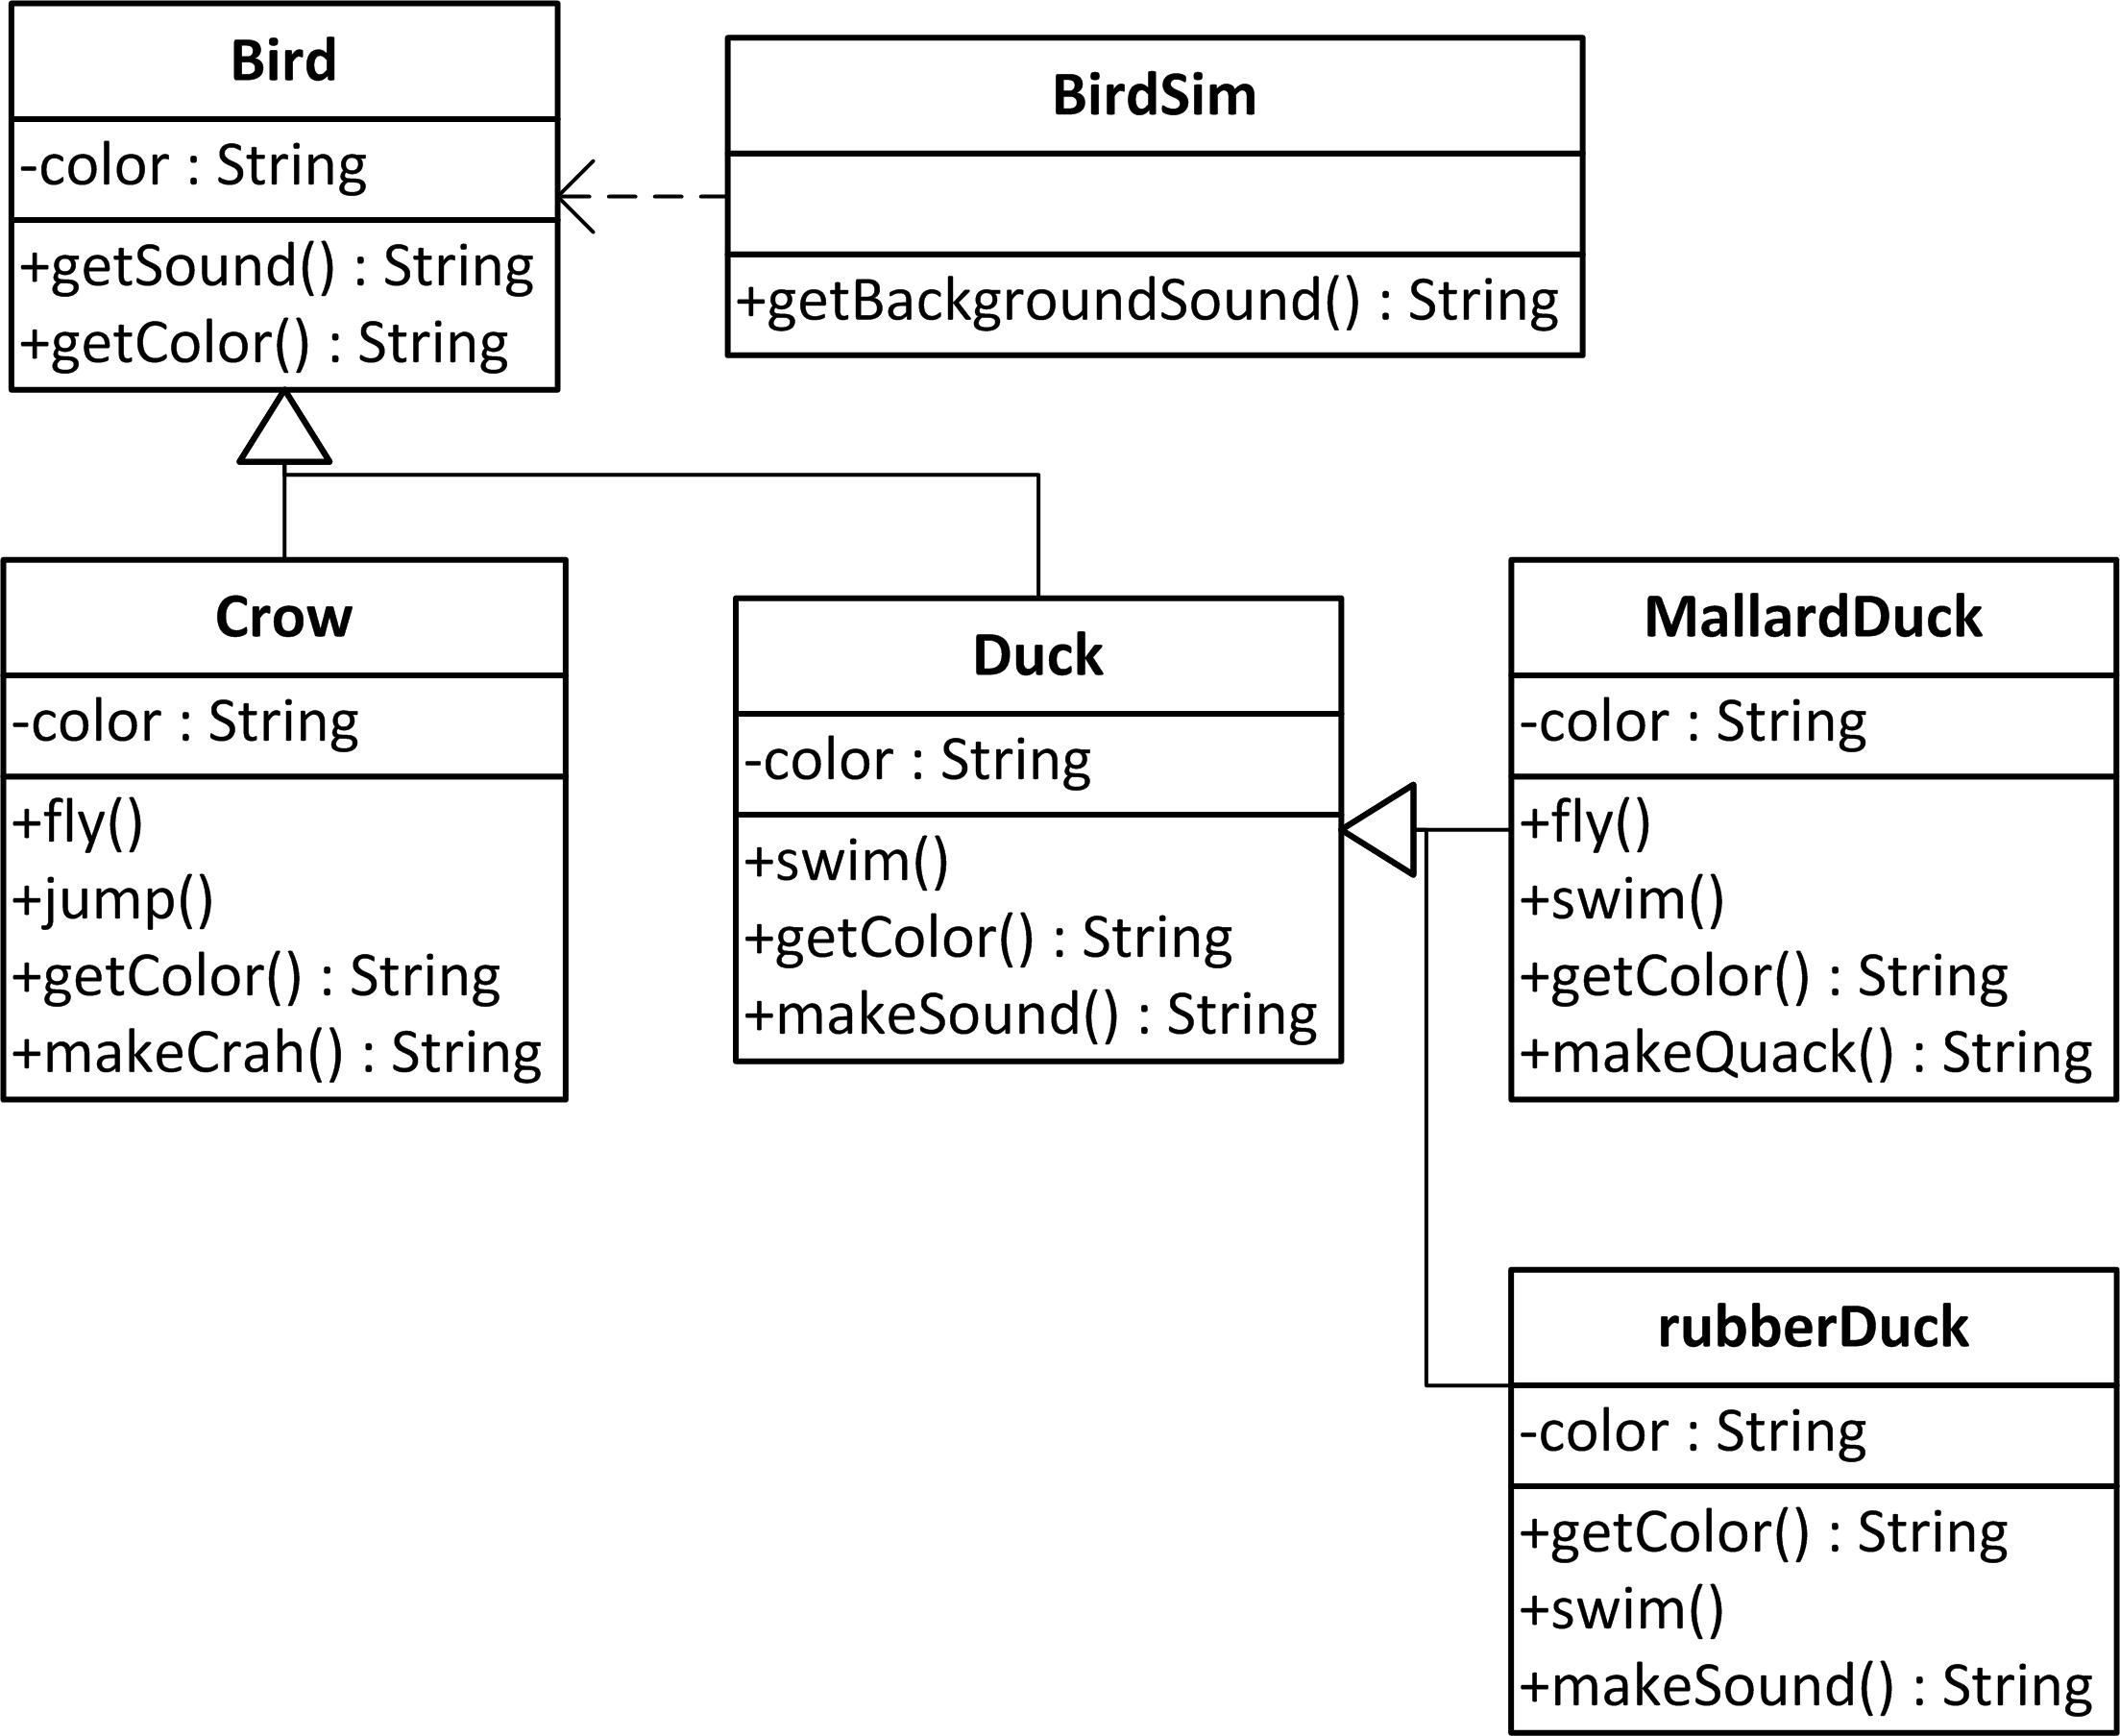
\includegraphics[scale=1]{bilder/uml/uml3.jpg}
\end{frame}

%%%%%%%%%%%%%%%%%%%%%%%%%%%%%%%%%%%%%%%%%%%%%%%%%%%%%%%%%%%%%%%%%%%%%%%%%

\begin{frame}{Vererbung - BirdSim}
	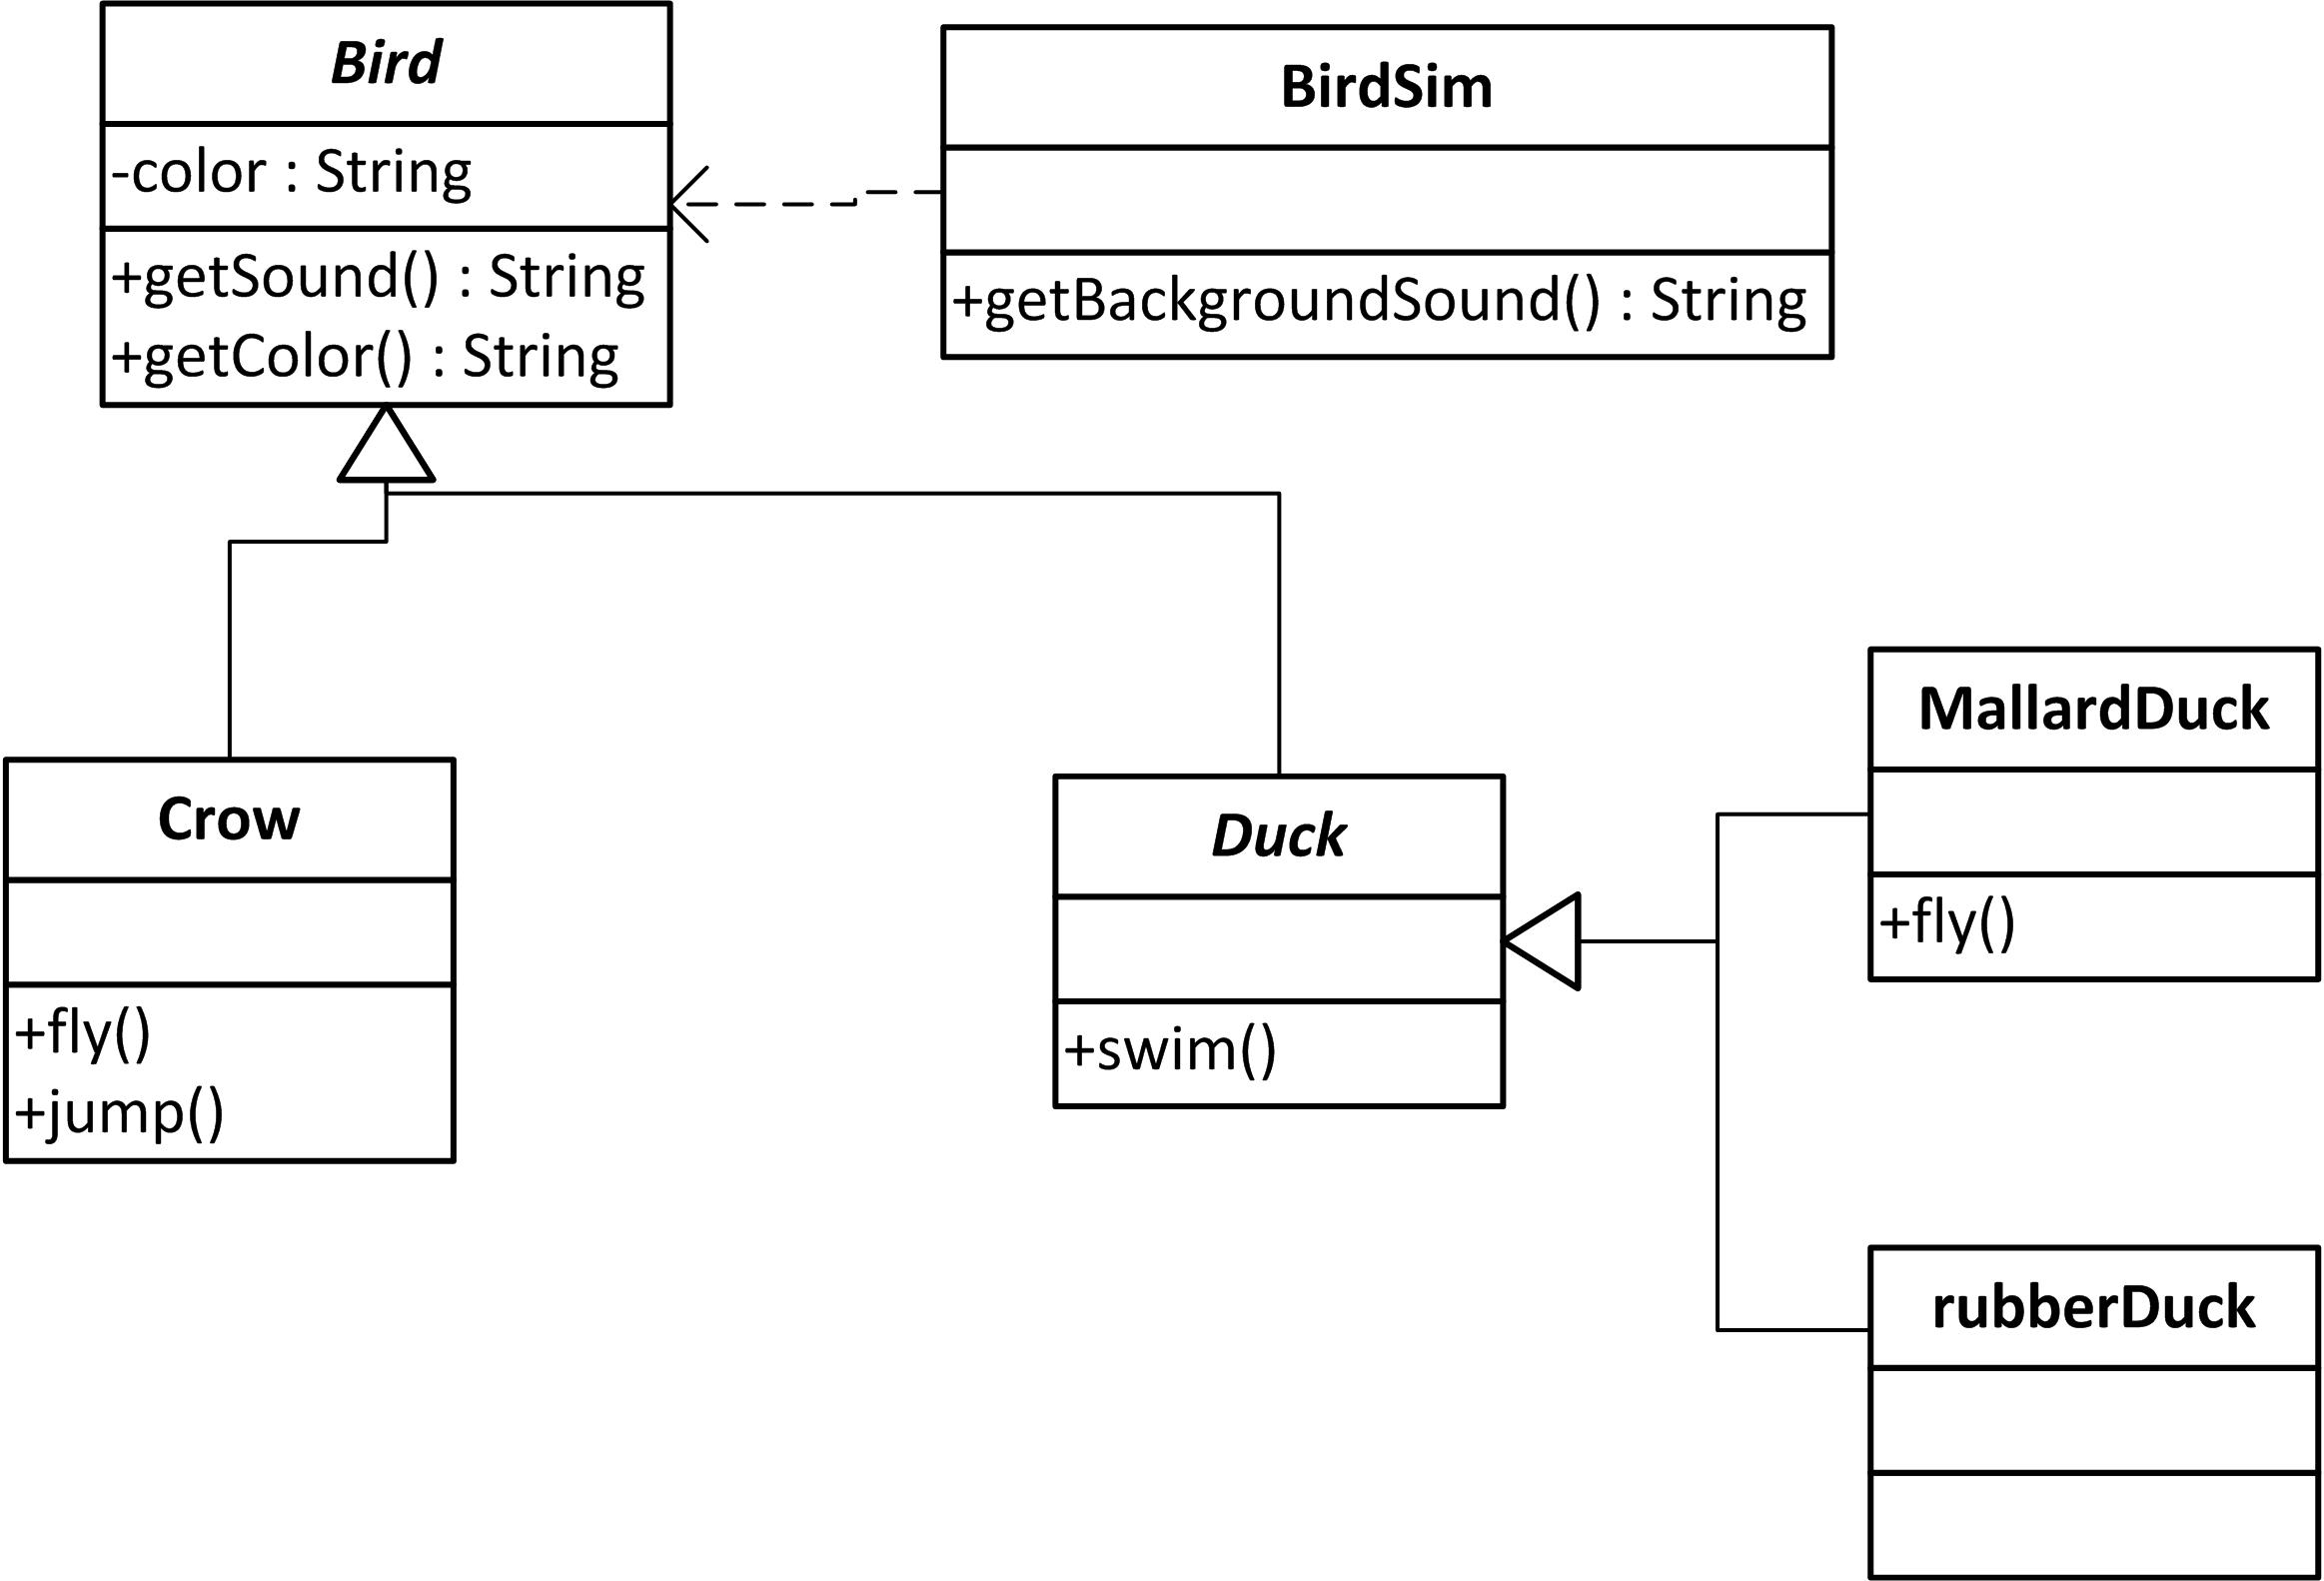
\includegraphics[scale=1]{bilder/uml/uml4.jpg}
\end{frame}

%%%%%%%%%%%%%%%%%%%%%%%%%%%%%%%%%%%%%%%%%%%%%%%%%%%%%%%%%%%%%%%%%%%%%%%%%
\subsection{Wie?}
\begin{frame}[containsverbatim]
	\frametitle{Vererbung - wie funktioniert's?}
	\emph{Bird.java}
	\begin{lstlisting}
public abstract class Bird {
	protected String color;

	public String getColor() {
		return color; 
	}
	
	public abstract String getSound(); //don't know which sound to create -> abstract
}
	\end{lstlisting}
	
	Die \emph{Bird}-Klasse ist allgemein gehalten. Wir wissen z.B. weder die konkrete Farbe des Vogels, noch das Geräusch, das er erzeugt. Trotzdem können wir definieren, dass ein Vogel eine Farbe hat und Geräusche machen kann.
\end{frame}

%%%%%%%%%%%%%%%%%%%%%%%%%%%%%%%%%%%%%%%%%%%%%%%%%%%%%%%%%%%%%%%%%%%%%%%%%

\begin{frame}[containsverbatim]
	\frametitle{Vererbung - wie funktioniert's?}
	\emph{Crow.java}
	\begin{lstlisting}
public class Crow extends Bird {
	public Crow() {
		color = "black";
	}

	public String getSound() {
		return "crah";
	}
}
	\end{lstlisting}
	
	\begin{itemize}
		\item Beim Erstellen einer Krähe wird festgelegt, dass sie schwarz ist
		\item \emph{getSound} wird \textbf{überschrieben}
	\end{itemize}
\end{frame}

%%%%%%%%%%%%%%%%%%%%%%%%%%%%%%%%%%%%%%%%%%%%%%%%%%%%%%%%%%%%%%%%%%%%%%%%%

\begin{frame}[containsverbatim]
	\frametitle{Vererbung - wie funktioniert's?}
	\emph{Duck.java}
	\begin{lstlisting}
public abstract class Duck extends Bird {
	public void swim() {
		//implementation of swimming
	}
}
	\end{lstlisting}
	
	\begin{itemize}
		\item \emph{Duck} erbt von \emph{Bird}
		\item trotzdem ist \emph{Duck} selbst auch \emph{abstract} (warum?)
		\item \emph{Duck} erweitert \emph{Bird} um eine weitere Methode: \emph{swim}
	\end{itemize}
\end{frame}

%%%%%%%%%%%%%%%%%%%%%%%%%%%%%%%%%%%%%%%%%%%%%%%%%%%%%%%%%%%%%%%%%%%%%%%%%

\begin{frame}[containsverbatim]
	\frametitle{Vererbung - wie funktioniert's?}
	\emph{BirdSim.java}
	\begin{lstlisting}
Bird[] myBirs;	
	
public BirdSim main(String[] args) {
	//create some Birds
	System.out.println(getBackgroundSounds());
}

public String getBackroundSound() {
	String result = "";
	for (int i = 0; i < myBirds.length; i++) {
		if (myBirds[i] != null) {
			result = result + myBirds[i].getSound();
		}
	}
	return result;
}
	\end{lstlisting}
\end{frame}

%%%%%%%%%%%%%%%%%%%%%%%%%%%%%%%%%%%%%%%%%%%%%%%%%%%%%%%%%%%%%%%%%%%%%%%%%
%%%%%%%%%%%%%%%%%%%%%%%%%%%%%%%%%%%%%%%%%%%%%%%%%%%%%%%%%%%%%%%%%%%%%%%%%
\subsection{Aufgabe.}
\begin{frame}{Vererbung - Aufgabe}
	\textbf{Aufgabe:} Schreibt je eine Klasse für \emph{MallardDuck} und \emph{RubberDuck} \pause
	
	\begin{enumerate}		
		\item Die Farben sollen festgelegt werden
		\item Sie sollen quaken/quietschen können
		\item \emph{MallardDuck} soll fliegen können
		\item Erweitert \emph{BirdSim}, sodass je eine \emph{MallardDuck}/\emph{RubberDuck} erzeugt und in das Array \emph{myBirds} hinzugefügt wird.
	\end{enumerate}
	
	\textbf{Soll-Ausgabe:} "crah, crah, quack, quietsch, "
\end{frame}


%%%%%%%%%%%%%%%%%%%%%%%%%%%%%%%%%%%%%%%%%%%%%%%%%%%%%%%%%%%%%%%%%%%%%%%%%
%%%%%%%%%%%%%%%%%%%%%%%%%%%%%%%%%%%%%%%%%%%%%%%%%%%%%%%%%%%%%%%%%%%%%%%%%
\subsection{Zusammenfassung}
\begin{frame}{Zusammenfassung}
	\begin{itemize}
		\item <spezielleKlasse> extends <allgemeineKlasse>
		\item Klassen können Eigenschaften und Methoden von genau einer anderen Klasse erben
		\item Es gibt allgemeine und spezialisierte Klassen \pause
		\item Allgemeine Klassen können \emph{abstract} sein
		\item Von \emph{abstract} Klassen kann man keine Instanzen erzeugen \pause
		\item Sichtbarkeit \emph{protected} bedeuted, dass erbende Klassen darauf zugreifen können
	\end{itemize}
\end{frame}

%%%%%%%%%%%%%%%%%%%%%%%%%%%%%%%%%%%%%%%%%%%%%%%%%%%%%%%%%%%%%%%%%%%%%%%%%
%%%%%%%%%%%%%%%%%%%%%%%%%%%%%%%%%%%%%%%%%%%%%%%%%%%%%%%%%%%%%%%%%%%%%%%%%
%%%%%%%%%%%%%%%%%%%%%%%%%%%%%%%%%%%%%%%%%%%%%%%%%%%%%%%%%%%%%%%%%%%%%%%%%

\section{Überladen von Methoden}
\subsection{Wozu / Wie?}
\begin{frame}[containsverbatim]
	\frametitle{Überladen - Wozu?}
	
	\emph{Calculator.java}
	\begin{lstlisting}
public int add2(int a, int b) {
	return a + b;
}

public int add3(int a, int b, int c) {
	return a + b + c;
}
	\end{lstlisting}

	\begin{itemize}
		\item add2 akzeptiert zwei Parameter
		\item add3 akzeptiert drei Parameter
	\end{itemize}		
\end{frame}

%%%%%%%%%%%%%%%%%%%%%%%%%%%%%%%%%%%%%%%%%%%%%%%%%%%%%%%%%%%%%%%%%%%%%%%%%

\begin{frame}[containsverbatim]
	\frametitle{Überladen - Wie?}
	
	\emph{Calculator.java}
	\begin{lstlisting}
public int add(int a, int b) {
	return a + b;
}

public int add(int a, int b, int c) {
	return a + b + c;
}
	\end{lstlisting}
	
	\textbf{Schöner:} Die Methode \emph{add} ist Überladen.
	
	Sie akzeptiert zwei \textbf{oder} drei int-Parameter!
\end{frame}

%%%%%%%%%%%%%%%%%%%%%%%%%%%%%%%%%%%%%%%%%%%%%%%%%%%%%%%%%%%%%%%%%%%%%%%%%

\begin{frame}[containsverbatim]
	\frametitle{Überladen - Wie?}
	
	\emph{Calculator.java}
	\begin{lstlisting}
public int add(int a, int b) {
	return a + b;
}

public int add(int a, int b, int c) {
	return add(add(a + b) + c);
}
	\end{lstlisting}
	
	Hier verwendet die überladene Methode die andere.
\end{frame}

%%%%%%%%%%%%%%%%%%%%%%%%%%%%%%%%%%%%%%%%%%%%%%%%%%%%%%%%%%%%%%%%%%%%%%%%%

\begin{frame}[containsverbatim]
	\frametitle{Überladen - Wie?}
	
	\emph{Calculator.java}
	\begin{lstlisting}
public int add(int a, int b) {
	return a + b;
}

public int add(int[] numbers) {
	int sum = 0;
	for (int i = 0; i < numbers; i++) {
		sum = add(sum, numbers[i]);
	}
	return sum;
}
	\end{lstlisting}
	
	Hier verwendet die überladene Methode ebenfalls die andere.
\end{frame}

%%%%%%%%%%%%%%%%%%%%%%%%%%%%%%%%%%%%%%%%%%%%%%%%%%%%%%%%%%%%%%%%%%%%%%%%%

\begin{frame}[containsverbatim]
	\frametitle{Überladen - Wie?}
	
	\emph{Calculator.java}
	\begin{lstlisting}
public Profile getProfile( int id) {
	//return a single profile
}

public Profile[] getProfile(int fromID, int toID) {
	//return a range of Profiles
}
	\end{lstlisting}
	
	Auch der Rückgabe-Wert kann verändert werden.
	
	
	Aber: Hier sollte man sich überlegen, ob die Trennung zu \emph{getProfile()} und \emph{getProfile\textbf{s}()} nicht besser wäre.
\end{frame}

%%%%%%%%%%%%%%%%%%%%%%%%%%%%%%%%%%%%%%%%%%%%%%%%%%%%%%%%%%%%%%%%%%%%%%%%%
%%%%%%%%%%%%%%%%%%%%%%%%%%%%%%%%%%%%%%%%%%%%%%%%%%%%%%%%%%%%%%%%%%%%%%%%%
\subsection{Aufgabe.}
\begin{frame}[containsverbatim]
	\frametitle{Überladen - Aufgabe.}

	\emph{Methoden}
	\begin{lstlisting}
public int add (int b, int c)
public String add (int a, double b)
public int add (int a, int b)
public int add (double a, int b);
	\end{lstlisting}
	
	\emph{Methodenaufrufe}
	\begin{lstlisting}
add(1, 1);
add(1.0, 1);
add(1, 1.0);
	\end{lstlisting}
	
	\begin{itemize}
		\item Welcher Aufruf ruft welche Methode auf?
		\item Wo ist der Fehler?	
	\end{itemize}
\end{frame}

%%%%%%%%%%%%%%%%%%%%%%%%%%%%%%%%%%%%%%%%%%%%%%%%%%%%%%%%%%%%%%%%%%%%%%%%%
%%%%%%%%%%%%%%%%%%%%%%%%%%%%%%%%%%%%%%%%%%%%%%%%%%%%%%%%%%%%%%%%%%%%%%%%%
%%%%%%%%%%%%%%%%%%%%%%%%%%%%%%%%%%%%%%%%%%%%%%%%%%%%%%%%%%%%%%%%%%%%%%%%%
\section{Aufgabenblatt}
\subsection*{Aufgabenblatt}
\begin{frame}{Aufgabenblatt}

\end{frame}

%%%%%%%%%%%%%%%%%%%%%%%%%%%%%%%%%%%%%%%%%%%%%%%%%%%%%%%%%%%%%%%%%%%%%%%%%
%%%%%%%%%%%%%%%%%%%%%%%%%%%%%%%%%%%%%%%%%%%%%%%%%%%%%%%%%%%%%%%%%%%%%%%%%
%%%%%%%%%%%%%%%%%%%%%%%%%%%%%%%%%%%%%%%%%%%%%%%%%%%%%%%%%%%%%%%%%%%%%%%%%
\section{Sortieren}
\subsection{Wozu?}
\begin{frame}{Sortieren - Wozu?}
	\textbf{Was bringt sortieren?}\pause
	
	Weil man dann schneller Sachen finden kann.
	
	$\rightarrow$ Binäre suche
\end{frame}

%%%%%%%%%%%%%%%%%%%%%%%%%%%%%%%%%%%%%%%%%%%%%%%%%%%%%%%%%%%%%%%%%%%%%%%%%
%%%%%%%%%%%%%%%%%%%%%%%%%%%%%%%%%%%%%%%%%%%%%%%%%%%%%%%%%%%%%%%%%%%%%%%%%
\subsection{Wie?}
\begin{frame}{Sortieren - Wie?}
		Es gibt sehr viele Sortieralgorithmen $\rightarrow$ VL Algorithmen 1
		
		Wir werden heute \emph{Insertionsort} auf einer einfach-verketteten Liste implementieren
\end{frame}

%%%%%%%%%%%%%%%%%%%%%%%%%%%%%%%%%%%%%%%%%%%%%%%%%%%%%%%%%%%%%%%%%%%%%%%%%

\begin{frame}{Insertionsort}
	\textbf{So funktioniert unser Insertionsort}
	
	Kopiere Elemente von einer unsortierten Liste so in eine neue Liste, dass diese dann sortiert ist:\pause
	\begin{enumerate}
		\item Suche \textbf{größtes} Element in unsortierter Liste ...
		\item ... und entferne es aus der unsortierten Liste...
		\item ... und füge es an den Anfang der sortierten Liste ein
		\item Fahr fort wie in (1), bis unsortierte Liste leer
	\end{enumerate}\pause
	
	\textbf{Frage:} Wie ist die neue Liste dann sortiert? Auf- oder Absteigend?
\end{frame}

%%%%%%%%%%%%%%%%%%%%%%%%%%%%%%%%%%%%%%%%%%%%%%%%%%%%%%%%%%%%%%%%%%%%%%%%%
%%%%%%%%%%%%%%%%%%%%%%%%%%%%%%%%%%%%%%%%%%%%%%%%%%%%%%%%%%%%%%%%%%%%%%%%%
\subsection{Aufgabe.}
\begin{frame}{Sortieren - Aufgabe.}
	\textbf{Aufgabe:} Schreibe eine Methode die eine Liste von Punkten sortiert. Punkte, die nah am Ursprung sind, 	sollen am Anfang der Liste stehen, weit entfernte am Ende.\pause
	
	
	Die Methode soll in der Klasse \emph{LinkedList} implementiert werden. Der Rückgabewert ist eine (neue) sortierte Liste.\pause
	
	
	\textbf{Tips:}
	\begin{itemize}
		\item \emph{distanceToOrigin}-Methode von \emph{Point} verwenden
		\item \emph{getPoint}-, \emph{addFirst}-, und \emph{remove}-Methode von \emph{LinkedList} verwenden
		\item Kein DeepCopy der \emph{Point}-Instanzen
	\end{itemize}
\end{frame}

\section{Zusammenfassung}
\subsection*{Was haben wir heute gemacht?}
\begin{frame}{Zusammenfassung}
	\textbf{Vererbung}
	\begin{itemize}
		\item ähnliche Klassen zusammenfassen
		\item abstrakte Methoden
		\item \emph{protected}-Schlüsselwort
	\end{itemize}
	
	\textbf{Überladen}
	\begin{itemize}
		\item selber Methodenname
		\item andere Signatur (Rückgabewert, Parameterliste)
		\item gegenseitige Verwendung
	\end{itemize}
	
	\textbf{Sortieren}
	\begin{itemize}
		\item schneller Dinge wieder finden
		\item Insertionsort
	\end{itemize}
\end{frame}

%Noch fragen Folie
\section{Fragen?}
\subsection*{Fragen} %Für das Design...
\begin{frame}	
	\begin{center}
		\huge{Fragen?}
	\end{center}
\end{frame}



%comic
\begin{frame}[full]

\includegraphics[scale=0.55]{bilder/comics/September-25-2011-18-44-59-aa71ce1bd67502c27bc56a6b8d724897.jpeg}
\end{frame}
\end{document}

\end{document}